\documentclass[12pt,a4paper]{article}
\usepackage[utf8]{inputenc}
\usepackage[finnish]{babel}
\usepackage{setspace}
%\usepackage{parskip}
%\usepackage{amssymb}
%\usepackage{amsmath}
\usepackage{graphicx}
\usepackage{subcaption}
\usepackage{fancyhdr}
\usepackage[top=1in, bottom=1in, left=1in, right=1in]{geometry}
\usepackage{float}
\usepackage[section]{placeins}
\usepackage[nottoc,notlot,notlof]{tocbibind}

\usepackage{titlesec}
\titleclass{\section}{top}
\newcommand\sectionbreak{\clearpage}
\titleformat*{\section}{\Huge\bfseries}
\titleformat*{\subsection}{\Large\bfseries}
\titleformat*{\subsubsection}{\large\bfseries}

%\usepackage[numbered,autolinebreaks,useliterate]{mcode}

\usepackage{siunitx}\sisetup{per=frac} % SI-yksiköitä.
%\usepackage{supertabular} % jos tarttee isoja taulukoita

\usepackage{hyperref}
\hypersetup{pdfborder={0 0 0}}
\onehalfspacing
\cfoot{}


\begin{document}

% Sisällysluettelo
\newpage
\thispagestyle{empty}
\tableofcontents
\newpage
\setcounter{page}{1}
\parskip=1em \advance\parskip by 0pt plus 2pt
\pagestyle{fancy}


%%%%%%%%%%%%%%% Oleellinen sisältö alkaa%%%%%%%%%%%%%%%
\section{Johdanto}



\cite{rj, yt, enzo}

%Teoreettista teoriaa. Täällä tarvitaan myös yhtälöitä, yhtälö \ref{esimerkkiyhtalo} on yksi sellainen.
%
%\begin{equation}\label{esimerkkiyhtalo}
%	c=\sqrt{a^2+b^2}
%\end{equation}

%\begin{align} % &-merkki kertoo mitkä kohdat laitetaan päällekkäin
%s_{1} =& d \cos \alpha = d \cos (90 \,^{\circ} - \varphi) = d \sin \varphi \label{align1} \\
%s_{2} =& d \cos \beta = d \cos (90 \,^{\circ} - \theta) = d \sin \theta \label{align2},
%\end{align}
%\begin{align}
%\lambda&=\frac s n \nonumber \\
%&= \frac{s_1-s_2}{n} \nonumber \\
%&= \frac{d}{n} ( \sin \varphi - \sin \theta ) \label{sievennystulos}
%\end{align}

%\begin{equation*}
%	\sin{x} \approx x \text{ kun x on pieni}
%\end{equation*}


\section{Enzo}
Enzo on mukautuvaa hilantihennystä (\textit{Adaptive Mesh Refinement}, AMR) hyödyntävä simulaatiokoodi, joka mahdollistaa aika- ja paikkaresoluution kasvattamisen simulaation kiinnostavilla alueilla. Tämä on tärkeää, sillä usein melko pienellä alueella tarvitaan suurta resoluutiota, mutta koko simulaation ajaminen näin suurella tarkkuudella veisi kohtuuttoman paljon aikaa.

	\subsection{Hila}
	Simuloitava alue katetaan kokonaan hilalla, jonka tiheys valitaan sellaiseksi, että saavutetaan pienin haluttava resoluutio. Tämä niinkutsuttu juurihila toimii juurena muiden hilojen muodostamalle hierarkialle, joka muodostuu, kun juurihilasta valitaan alueita simuloitavaksi korkeammalla resoluutiolla.\cite{enzo}
	
	Kaikki hilat ovat karteesisia ja suorakulmaisia. Alueille, joilla tarvitaan korkeampaa resoluutiota, asetetaan juurihilan kanssa päällekkäin toinen, hienorakeisempi hila. Näitä sisäkkäisiä hiloja voi tarvittaessa olla teoriassa mielivaltaisen monta ja ne muodostavat puumaisen rakenteen.\cite{enzo}%oikeasti mielivaltaisen monta?
	%Alueet, joilla käytetään suurempaa resoluutiota, valitaan siten, että niiden kaikki tahkot ovat päällekäin jonkin matalamman resoluution hilan tahkojen kanssa. 
	
	Kullakin hilalla juurihilaa lukuun ottamatta on vanhempi, joka sisältää hilan kokonaan. Yhdellä hilalla voi olla useita lapsia, mutta aina vain yksi vanhempi. Tavallisesta puita koskevasta nimeämiskäytännöstä poiketen sisaruksiksi kutsutaan kaikkia niitä hiloja, joiden resoluutio on sama eli ne sijaitsevat puussa samalla tasolla.\cite{enzo}
	
	Hienompia hiloja luotaessa valitaan hilan solujen koko siten, että hila rajoittuu reunoistaan vanhempansa solujen tahkoihin. Lisäksi solun vanhemman sivun pituuden tulee olla jokin monikerta solun sivun pituudesta.  

%Siksi AMR-simulaatioissa 

%Esimerkiksi kuvassa \ref{fig:enzogrid} nähdään, kuinka tiheämmillä alueilla käytetään pienempiä 

\begin{figure}
   \centering
   \begin{subfigure}[b]{0.45\textwidth}
       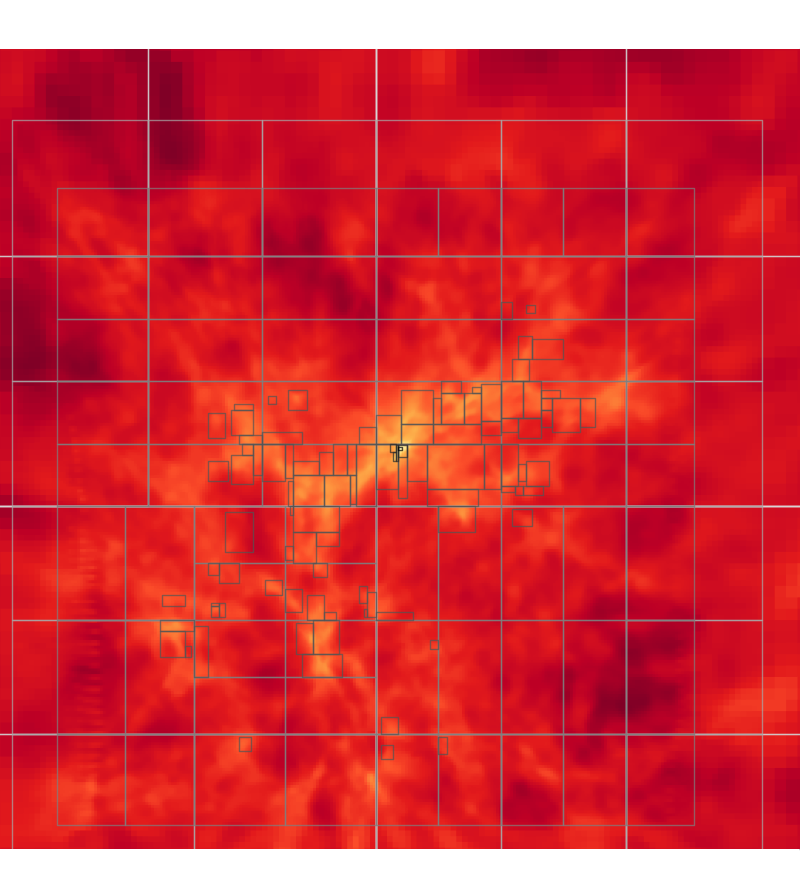
\includegraphics[height=7.9cm]{../kuvat/amr-grid.png}
   \end{subfigure}
   \begin{subfigure}[b]{0.45\textwidth}
       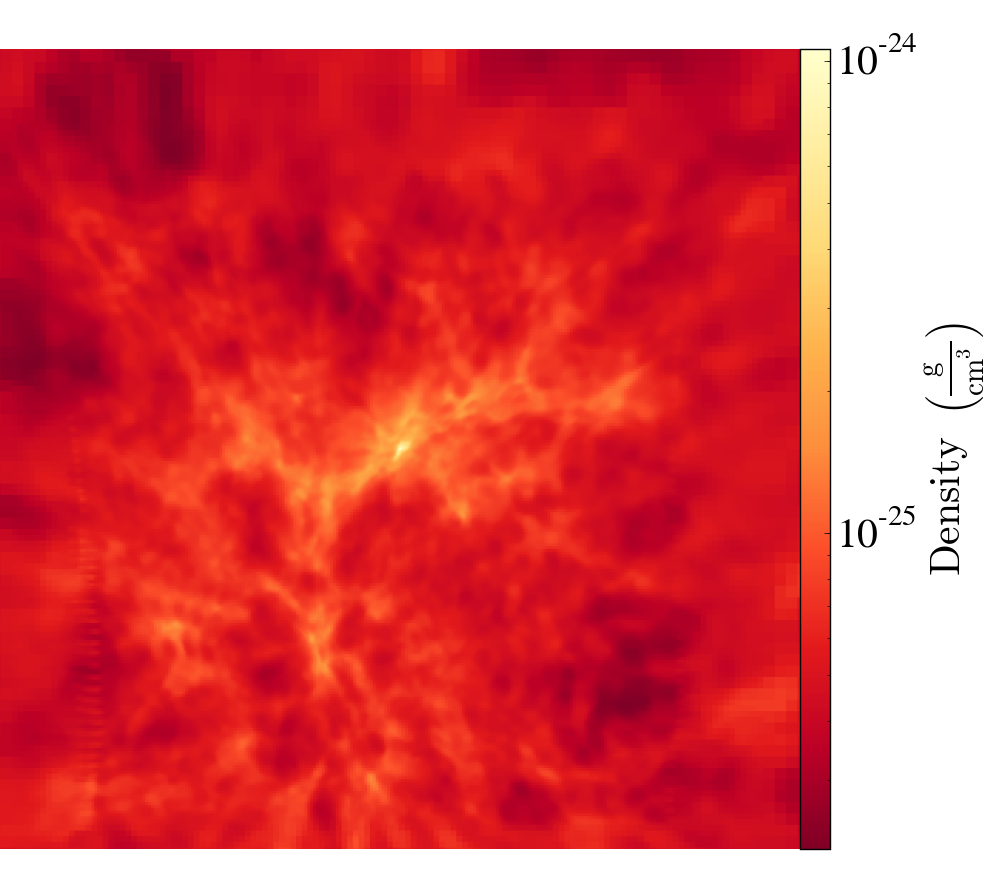
\includegraphics[height=7.9cm]{../kuvat/amr-nogrid.png}
   \end{subfigure}
   \caption{Halkileikkaus $100$ pc$^2$ alueesta eräästä Enzo-simulaatiosta solujen rajat näkyvillä (vasen kuva) sekä ilman niitä (oikea kuva). Kiinnostavammilla alueilla solut ovat pienempiä. Resoluution heikentyminen suuremmissa soluissa on selvästi nähtävissä.}\label{fig:enzogrid} %TODO mieti: miten näkyviin se, että kyseessä on Johnin simulaatio? Kerro mitä kuvassa on

\end{figure}

\section{\texttt{yt}}
waaaiiiitiiii

%\begin{figure}
%\centering
%\includegraphics[width=\textwidth]{yllatyskipsu.jpg} %lveydeksi voi antaa myös vaikkapa 5cm tai muun konkreettisen mitan tai vaihtoehtoisesti asettaa leveydeksi vaikapa 80% tekstin leveydestä parametrilla 0.8\textwidth. Kuvan korjeuden voi asettaa esimerkiksi height=6cm.
%\caption{Kuvatekstissä voisin vaikkapa kertoa, että oikeasti kissa vain haukottelee.}
%\label{kissakuva}
%\end{figure}

\section{Oma työ}
joo kyl mäki tein jotain


\section{Tulokset}
tulostan tähän tuloksia


\section{Loppupäätelmät}
paska työ mutta tulipahan tehtyä


%%%%% Sisältö loppuu, lähdeluettelo %%%%%
\bibliographystyle{plain}
\bibliography{lahteet}

\appendix
\newpage
\section{Liittyvä liite.} \label{koodi}
Liian laaja leipätekstiin.
\end{document}
